\documentclass[14pt,a4paper]{article}

\usepackage[utf8]{inputenc}
\usepackage[russian]{babel}
\usepackage[left=1.5cm,right=1.5cm,top=2cm,bottom=2.5cm]{geometry}
\usepackage{setspace}
\usepackage{indentfirst}
\usepackage{amssymb}
\usepackage{amsmath}
\usepackage{array}
\usepackage{amsfonts}
\usepackage{dashbox}
\usepackage{colortbl}
\usepackage[fontsize=14pt]{scrextend}
\usepackage{tabularx}
\usepackage{graphicx}
\graphicspath{{img/}}
\usepackage{fancyvrb}
\usepackage[unicode, pdftex]{hyperref}
\usepackage{color,colortbl}
\renewcommand{\baselinestretch}{1.3}
\usepackage[Glenn]{fncychap}
\usepackage[usenames,dvipsnames,svgnames,table]{xcolor}


%\pagecolor[HTML]{111111} % dark color
%\color[HTML]{EEEEEE} % light color

\usepackage{cmap} % для кодировки шрифтов в pdf
\usepackage{amssymb}
\usepackage{amsmath}

\usepackage{mathrsfs}
\usepackage{mathrsfs}
\usepackage{amsfonts}

\usepackage{amsmath}

% для многострочных комментариев
\usepackage{verbatim}
\definecolor{mygray}{rgb}{0.4,0.4,0.4}
\definecolor{mygreen}{rgb}{0,0.8,0.6}
\definecolor{myorange}{rgb}{1.0,0.4,0}


\newcommand{\HRule}{\rule{\linewidth}{0.5mm}}

\begin{document}

% \documentclass{report}
% \usepackage[russian]{babel}
% \usepackage[utf8]{inputenc}
% \usepackage[pdftex]{graphicx}

% \begin{document}

  \begin{titlepage}
  % ============== %
    \begin{center}
      
\includegraphics{img/msu_logo.jpg}
      \normalsize
      \\[0.1cm]
      Московский государственный университет имени М.В.Ломоносова
      \\[0.1cm]
      Факультет вычислительной математики и кибернетики
      \\[0.1cm]
      Кафедра вычислительных технологий и моделирования
      \\[1.5cm]
      {\Large Кирякин Максим Валерьевич}
      \\[1.0cm]
      \textbf{\Large Применение компартментно-сетевых моделей для моделирования эпидемического процесса }
      \\[1.0cm]
      Выпускная квалификационная работа
      \\[4.0cm]
      \begin{flushright}
      	\normalsize
         \textbf{Научный руководитель:}
         \\
         д.ф.-м.н., профессор Романюха А.А.
         \\
         \textbf{Со-руководитель:}
         \\
          к.ф.-м. н. Санникова Т.Е.

      \end{flushright}
      \vfill 
      Москва, 2024
    \end{center} 
  \end{titlepage}

% \end{document}


\newpage
\tableofcontents

\newpage
\section{Введение}

Сетевые модели играют важную роль в моделировании распространения инфекций, таких как эпидемии и пандемии различных заболеваний. Использование сетевых моделей позволяет учитывать сложные взаимодействия между индивидами, их перемещения и контакты, что позволяет более точно оценить потенциальное распространение заболевания и принять эффективные меры по его контролю и предотвращению. В данной работе рассматривается применение сетевых моделей для изучения динамики распространения инфекций в зависимости от свойств сети контактов.

Целью этой работы является на основе анализа демографических данных построить и исследовать модель распространения инфекции.

\textbf{Задачи работы:}
\begin{itemize}
	\item Собрать и проанализировать данные по возрастно-половому составу населения, распределению размеров домохозяйств, предприятий, учебных заведений.
	
	\item  По собранным данным разработать алгоритм построения сети контактов, которая будет обладать теми же характеристиками, что и основная популяция.
	
	\item Разбить популяцию на группы исходя из среднего числа контактов человека. Для каждый группы выполнить моделирование распространения инфекции с помощью модели SIR.
	
	\item Провести эксперименты по установлению динамики распространения инфекции в зависимости от типа популяции, наличия локдауна и величины параметров SIR модели.
	
\end{itemize}



\section{Сетевой подход}

На сегодняшний день при исследовании реляционных отношений между объектами социума все чаще начинают использоваться сетевые модели. Особую известность этот подход получил в области здравоохранения, при моделировании распространения инфекций, передающихся воздушно-капельным или половым путем \cite{network_analysis}.

Всего можно выделить 4 важных особенности сетевой парадигмы:
\begin{itemize}
	\item подход преимущественно фокусируется на отношениях между субъектами, а не на отношениях между их атрибутами.
	
	\item в основе подхода лежат имперические данные.

	\item подход часто использует математические и вычислительные модели.
	
	\item сам подход можно назвать графичным и репрезентативным.
\end{itemize}

Традиционные подходы моделирования в области здравоохранения часто предполагают, что можно получить данные на уровне отдельного человека. В этом случае еще до начала эксперимента согласно установленным критериям проводится опрос кандидатов, а уже потом начинается моделирование. Так, например, если мы хотим собрать данные среди учеников школы, у нас будет таблица размерами N на k, где каждый из N учеников будет опрошен по k атрибутам. 
Таким образом, точная модель сети контактов требует знания каждого человека в
популяции и каждого контакта между людьми, вызывающего
заболевание. Даже для небольших
групп населения это обычно неосуществимо, поэтому обычно приходится работать с приблизительными сетями. Существует несколько
методов сбора информации, для построения моделей контактной сети, приближенной к реальной. Они включают в себя
отслеживание всех инфицированных лиц и их контактов во время
или после вспышки \cite{Klovdahl}, обследование
отдельных лиц в популяциях \cite{Eubank}, а также
использование переписи населения \cite{Meyers},
социальных характеристик \cite{Meyers} или другие собранные данные \cite{Meyers_2003}.


Таким образом, возвращаясь к примеру со школой, при сетевом подходе сеть строится до начала сбора данных о контактах, поэтому на выходе получается таблица размерами N на N, где каждая ячейка с индексами $i, j$ ($i, j \in \overline{1, N}$)содержит информацию о контакте между двумя людьми с соответствующими индексами. 


При построении сети контактов исследователи часто уделяют особое внимание модели <<малого мира>> (small-world networks, \cite{Watts}), которая характеризуется высоким уровнем локальной кластеризации и глобальной связности. Такие модели могут использоваться при создании сети контактов для небольших групп, например, внутри рабочих коллективов, школ и университетов. Помимо этого также широко используются безмасштабные сети \cite{BA}, характеризующиеся степенным распределением.
К таким сетям можно отнести сеть Интернет \cite{www} или, например, белковые взаимодействия \cite{Wuchty}.


\subsection{Анализ данных}

После того, как сеть контактов построена, можно переходить к анализу собранных данных. Здесь существуют несколько основных подходов. Во-первых, большую роль в исследовании играет визуализация полученных данных. На сегодняшний день существует много программных пакетов, которые позволяют изобразить сеть контактов в понятном виде. Во-вторых, используют описательный анализ свойств сети. В этом случае сеть рассматривается как граф, на котором рассчитываются интересующие исследователей метрики. В-третьих, сейчас активное распространение получают стохастические методы. Так в последние десятилетия были разработаны стохастические методы сетевого моделирования, которые могут использоваться для проверки сетевых гипотез. Все эти подходы более детально рассмотрены в статье \cite{network_analysis}. 

\subsection{Сети передачи}

После формирования и анализа сети, приступают к моделированию передачи каких-либо структурных элементов по этой сети. Такие сети называют сетями передачи \cite{network_analysis}. При этом есть два основных типа сетей передачи: сети передачи болезней и сети передачи информации. В случае моделирования растпространения инфекций эпидемическая модель, построенная на основе сетей является наиболее полезной для определения хода вспышки или эпидемии. Так как именно сетевая модель раскрывает структуру передачи инфекции, позволяет анализировать взаимодействия объектов сети. Кроме этого, сетевая модель крайне полезна при планировании мероприятий по борьбе с этими заболеваниями.  


\subsection{Использование математических моделей при сетевом анализе}

Одним из способов моделирования является разбиение людей в популяции на группы, исходя из их среднего числа контактов друг с другом в течение дня. При таком подходе группы получаются достаточно однородные, и становится возможным использовать на них математические подходы, для которых требование однородности выборки является критичным (также говорят, что такая выборка удовлетворяет условиям гомогенного смешивания).

При создании алгоритма, который мог бы проводить такой расчет, нужно прежде всего как можно точнее задать начальные параметры. На сегодняшний день исследований, которые бы содержали такую информацию для жителей России не так много. Одним из таких исследований, является опрос, проведенный среди жителей Томска \cite{Tomsk}. В ходе опроса людям предлагалось заполнить бланк, в котором нужно было указать, сколько контактов с другими людьми у них было в тот день. Всем участникам было объяснено, в каком формате надо было давать ответы, поэтому полученные данные являются достаточно точными. В статье авторы определяют контакт как диалог меду людьми, состоящий минимум из 5 слов, при условии, что два человека находятся рядом друг с другом. Всего в ходе исследования было опрошено 505 человек. Полученную выборку людей нельзя считать репрезентативной с точки зрения расперделения по возрасту и полу, так как большей частью опрешенных были студенты. Однако в исследовании были получены хорошие данные для контактов, например, внутри домохозяйств, школ и предприятий. 




\subsection{SIR модель. Основные понятия}

В данной работе процесс распространения инфекции моделируется с помощью компартментно-сетевых моделей. То есть каждому человеку в популяции в каждый момент времени присвоено какое-то конкретное состояние из заданного набора. При таком подходе динамика распространения инфекции может быть описана с помощью классической SIR модели \cite{Murray}. В этом случае каждый индивид может иметь только одно из трех состояний:

\begin{itemize}
		
 \item восприимчивый (susceptible) -- описывает людей, которые могут заразиться инфекцией.
 \item зараженные (infectious) -- описывает людей, которые в текущий момент времени заражены и могут распространять инфекцию.
 \item выздоровевший (removed) -- описывает людей, которые обладают иммунитетом к болезни, так как недавно переболели или были вакцинированны.
  
\end{itemize}
    
Каждая категория может быть представлена в виде функции, зависящей от времени. При этом предполагается, что все три величины связаны друг с другом с помощью условия-нормировки:

\begin{equation}
S(t) + I(t) + R(t) = 1
\end{equation}

При такой постановке задачи система, описывающая распространение инфекции, имеет следующий вид:
\begin{equation}
	\begin{cases}
		\frac{d S}{d t} = -\lambda \beta_0 I S, \\
		\frac{d I}{d t} = -\mu I + \lambda \beta_0 I S, \\
		\frac{d R}{d t} = \mu I .
	\end{cases}
	\label{eq:SIR_system_base}
\end{equation}

Процесс, заданный системой, можно описать так:  инфицированные люди переходят в группу здоровых со скоростью $\mu$, в то время как восприимчивые переходят в класс зараженных со скоростью, пропорциональной плотностям I и S. Здесь $\lambda$ -- это коэффициент распространения инфекции для заданной группы людей, а $\beta_0$ -- параметр распространения, который считается постоянным для всей популяции.
 
Одним из основных параметров, которые отвечают за распространение инфекции, является базовое репродуктивное число $R_0$. Он описывает, сколько людей может заразить один инфицированный человек, при условии, что все остальные люди в популяции являются восприимчивыми. В предоположении однородности выборки, этот базовое репродуктивное число может быть найдено следующим образом:

\begin{equation}
	R_0 = \frac{\beta}{\gamma}
\end{equation}


\subsection{SIR модель для сложных сетей}

При моделировании сетей с большим числом людей, мы предполагаем, что каждый узел в сети -- это человек, а каждая его связь -- это возможный путь, по которому может передаваться инфекция. В данной парадигме можно считать, что $\lambda_k$ -- это вероятность, с которой человек с числом контактов k может быть заражен, если у него есть связи с инфицированными людьми. В то же время, каждый зараженный человек с вероятностью $\mu$ переходит из категории зараженного в категорию выздоровевшего. Этот параметр без потери общности можно положить равным единицы.

Так как теперь мы полагаем, что моделирование идет в рамках заданных групп, функции $R(t)$, $I(t)$, $S(t)$ будем считать различными для каждой группы и введем для них индекс группы: $R_k(t)$, $I_k(t)$, $S_k(t)$.

Таким образом, условие нормировки для каждой группы будет иметь вид:
\begin{equation}
	S_k(t) + I_k(t) + R_k(t) = 1
\end{equation}

При таких обозначениях система \eqref{eq:SIR_system_base} примет вид:
\begin{equation}
	\begin{cases}
		\frac{d S_k}{d t} = -\lambda_k \beta_0 I_k S_k, \\
		\frac{d I_k}{d t} = -\mu I_k + \lambda_k \beta_0 I_k S_k, \\
		\frac{d R_k}{d t} = \mu I_k .
	\end{cases}
	\label{eq:SIR_system_base_groups}
\end{equation}



\section{Сбор и анализ даных}

В ходе работы был произведен сбор данных относительно возростно-полового состава населения, в зависимости от региона страны. Кроме того, так же были проанализированы такие факторы, как число предприятий, размер домохозяйств, число школ, доли работающего населения по регионам. Информация собиралась не только по городам, но и по сельской местности.

\subsection{Численность населения}\label{1}

Для анализа с сайта федеральной службы государственной статистики \cite{rosstat} были взяты данные о числе жителей по возрастным категориям. В результате были определены коэффициенты для городского и сельского населений (Приложения. Таблица \ref{coeff}), которые далее использовались для создания синтетической популяции. Число мужчин и женщин в при этом предлагается рассчитываться по формуле:

\begin{equation}
	{}_n N_x = \alpha_{\text{тип популяции}}^{\text{пол}} \cdot N_{\text{тип популяции}}^{\text{пол}}, 
\end{equation}
где:
\begin{itemize}
	
	\item $n$ -- ширина группы.
	
	\item $x$ -- начало интервала.
	
	\item $\alpha_{\text{тип популяции}}^{\text{пол}}$ -- коэффициент пропорциональности для мужчин и женщин в зависимости от типа популяции. 
	
	\item $ N_{\text{тип популяции}}^{\text{пол}}$ -- размер выборки для мужчин и женщин в синтетической популяции в зависимости от типа популяции.
	
	
\end{itemize}

По обработанным данным были составлены возрастные пирамиды (Рисунок \ref{fig:tree}).

\begin{figure}[h!]
	\centering
	
\includegraphics[width=1\textwidth]{img/tree_theory.png}
	\caption{Возрастные пирамиды для сельского и городского населений.}
	\label{fig:tree}
\end{figure} 

На графике можно видеть, что распределение по возрастам имеет бимодальное распределение. Это может быть связано с тем, что в $90$-е годы в связи с тяжелой обстановкой в стране была низкая рождаемость. Так же можно предположить, что просадка обусловлена высокой миграцией молодого населения в те годы. Отдельно можно отметить тот факт, что женщин пожилого возраста больше, чем мужчин как в сельском, так и в городском населении.







\subsection{Предприятия}\label{3}


При построении модели синтетической популяции особое внимание уделялось предприятиям, так как именно на них приходится значительная часть контактов между агентами. Для того, чтобы получить достоверные данные о предприятиях, было проанализировано количество государственных бюджетных учреждений в различных регионах России. При анализе учитывались не только организации, созданные Российской Федерацией и её субъектами, но и муниципальные образования. Таким образом, удалось учесть взаимодействие агентов в различных сферах, таких как наука, образование, здравоохранение, культура, социальные услуги и другие важные области.


Согласно полученным данным, государственные учреждения распределены по регионам России достаточно равномерно (кроме Москвы). Наибольшее количество таких учреждений находится в Московской области ($1828$ штук), в то время как Республика Карелия имеет самое маленькое количество государственных учреждений среди всех регионов -- всего лишь $90$. Этот факт указывает на неравномерность экономического развития регионов, что необходимо учитывать при создании синтетической популяции.

Из данных было установлено, что Московская область сильно отличается по показателям от других областей. Поэтому для анализа того, сколько человек в среднем приходится на одну организацию использовали медиану, так как она не чувствительна к выбросам в данных. 

\subsection{Школы}\label{4}

Отдельно в работе были рассмотрены школы, так как  они является важным элементом общества не только с точки зрения распространения инфекций, но и с точки зрения использования для моделирования различных социальных сценариев, таких как изменение групповой динамики, исследование влияния различных факторов на качество образования и т.д. На графике \ref{fig:schools} приведено количество школ для сельского и городского населений для основных регионов России.


\begin{figure}[h!]
	\centering
	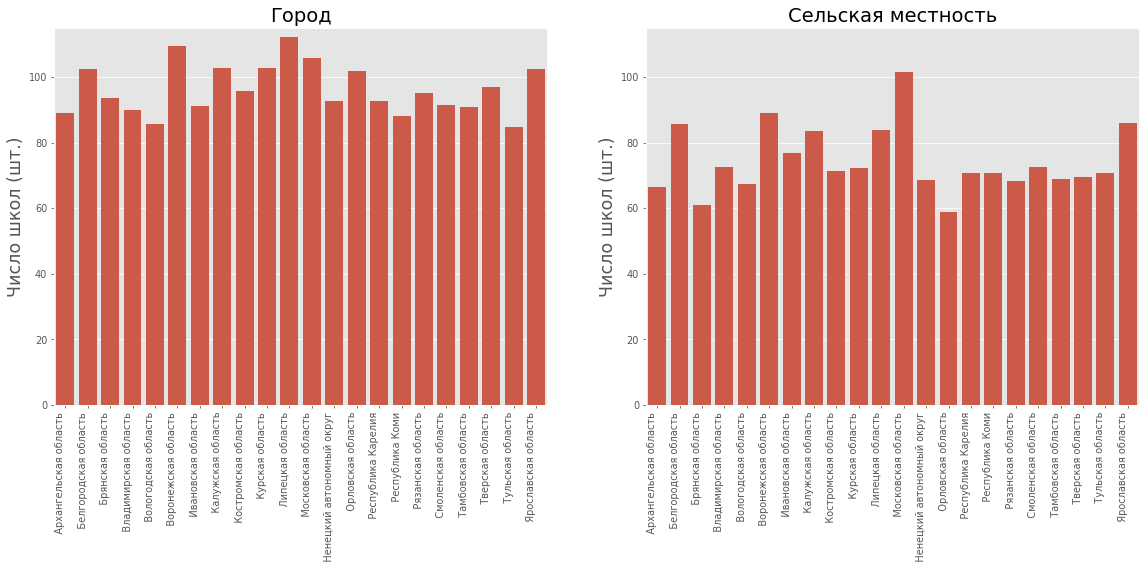
\includegraphics[width=1.0\textwidth]{img/schools.png}
	\caption{Количестко школ по субъектам Российской Федерации.}
	%\caption{Число школ по областям для города и сельской местности}
	\label{fig:schools}
\end{figure}


Из графика видно, что в сельской местности школ меньше чем в городе. При этом 
было рассчитано, что в среднем для сельского населения на одну школу приходится $18205$ человек, для городского -- $14689$.

\subsection{Число людей в домохозяйствах}\label{5}

При создании синтетической популяции необходимо знать чило домохозяйств и их размеры. Это поможет создать более точную и реалистичную сеть контактов, а так же лучше моделировать распространение инфекции. На основе данных росстата \cite{rosstat} были получены доли для каждого размера домохозяйств (Рисунок \ref{fig:households_theory}). Полученные значения, были использованны при дальнейшем моделировании и приведены в таблице \ref{tab: 111}. 


\begin{figure}[h!]
	\centering
	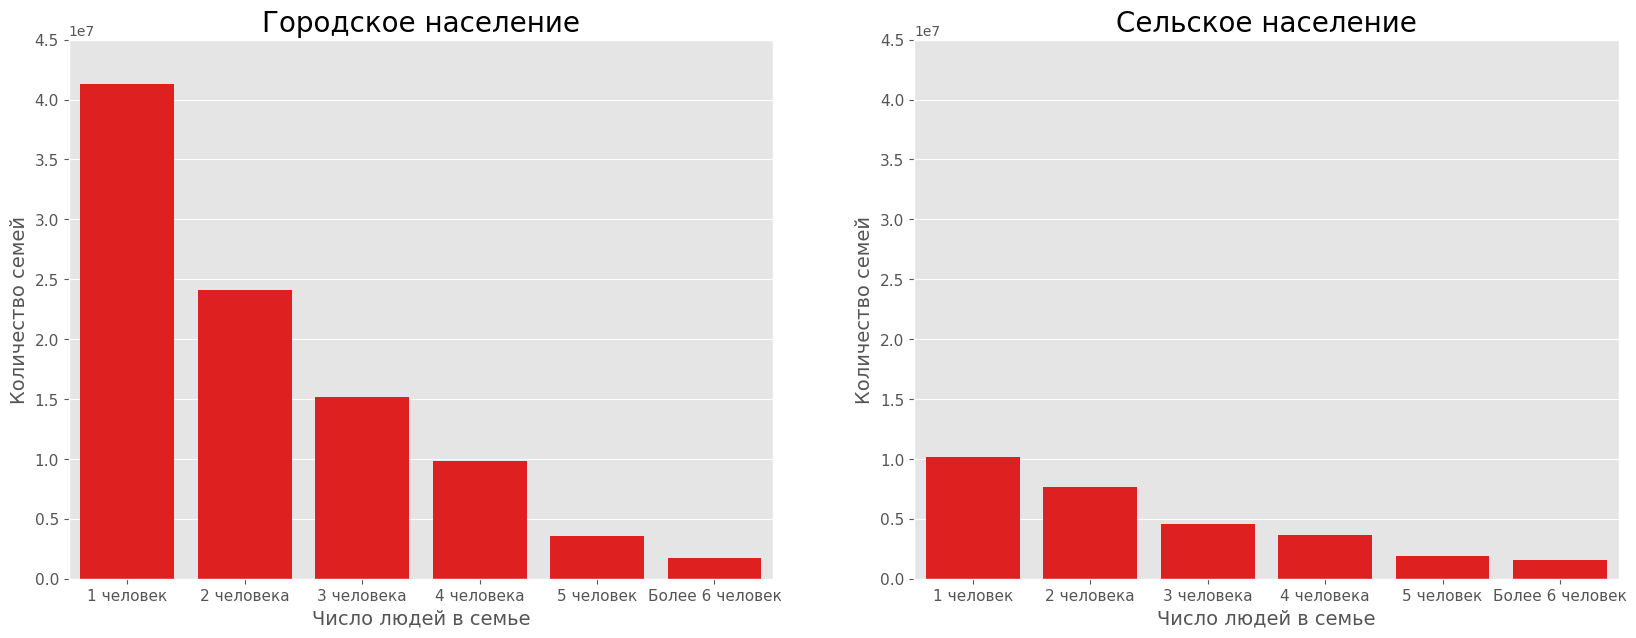
\includegraphics[width=1.0\textwidth]{img/households_distibution_theory.png}
	\caption{Распределение домохозяйств по размерам.}
	\label{fig:households_theory}
\end{figure}


%Можно видеть, что в выбранных для анализа областях преобладают домохозяйства из двух человек. При этом на домохозяйства из трех человек приходится примерно треть от общего числа. 


\section{Алгоритм создания сети контактов}

В ходе работы была написанная программа на языке Python \cite{github}, которая позволила создать сеть контактов с нужными характеристиками и провести на ней ряд экспериментов. Всего работу программы можно разбить на три основных этапа: считывание и предобработка необходимых для моделирования данных, создание на их основе синтетической популяции, моделирование распространения инфекции с помощью SIR модели на подгруппах полученной популяции.
Рассмотрим каждый этап более детально:

\textit{Считывание и предобработка данных.} Все данные были взяты в сайта росстата \cite{rosstat} и представленны в виде сгруппированных excel файлов, которые поступают на вход программы. Данные рассматривались в разрезе сельского и городского населений. К этим файлам относятся: 

\begin{itemize}

\item age\_sex\_distribution\_percentage.xlsx -- файл представляет из себя таблицу (сслыка), в которой указано, сколько процентов от всей популяции составляют люди каждой возрастной группы. При этом в возрастную группу входит сразу 5 возрастов (например, от 0 до 4, от 5 до 9 и тд). Отдельно рассматривается группа людей возрастом 70 лет и более. 
\item  households.xlsx -- файл содержит размеры домохозяйств для всех регионов страны. Данные представленны в таблице (ссылка).
\item  manufactures.xlsx -- файл содержит информацию о числе предприятий разных видов для каждой области. Данные представленны в таблице (ссылка).
\item  schools.xlsx -- файл содержит информацию о том, сколько школ приходится на каждую область. Данные представленны в таблице (ссылка).

\end{itemize}

\textit{Создание синтетической популяции}. Данный этап является самым сложным и ресурсозатратным. После его завершения формируется таблица с популяцией и матрица контактов для нее. Возможные столбцы таблицы с популяцией и их допустимые значения приведены в таблицу \ref{fig:table_paremeters_population}

\begin{table}[h]
	\centering
	\begin{tabularx}{\textwidth}{|c|X|}
		\hline
		Параметр               & Допустимые значения                                         \\
		\hline
		Id                     & целочисленное значение (integer). -1 если не заполнено      \\
		Возраст                & целочисленное значение (integer). -1 если не заполнено      \\
		Пол                    & male/female                                                 \\
		Id домохозяйства       & целочисленное значение (integer). -1 если не заполнено      \\
		Социальная роль        & ребенок/родитель/не имеет детей                             \\
		Тип популяции          & rural/urban                                                 \\
		Номер предприятия      & целочисленное значение (integer). -1 если не заполнено      \\
		Номер университета     & целочисленное значение (integer). -1 если не заполнено      \\
		\hline
	\end{tabularx}
	\caption{Таблица допустимых значений параметров для популяции.}
	\label{fig:table_paremeters_population}
\end{table}

Матрица контактов представляет из себя квадратную матрицу, которая хранится в памяти в разряженном формате, и содержит информацию о взаимодействии между людьми. При этом в ячейке с индексами i, j содержится 1, если люди с такими id имели контакт, и 0 в противном случае. 

Сам этап создания популяции так же можно разбить на несколько подэтапов. Сначала рассчитывается, сколько людей должно приходиться на каждую возрастную группу для каждого типа популяции, эти вычисления проводятся на основании загруженных ранее шаблонов. Далее создается популяция, где каждому человеку проставляются его основные атрибуты, которые можно задать на данном этапе (возраст, пол, тип популяции, id). 

После этих шагов необходимо сформировать домохозяйства. Это делается на основе данных, собранных на первом этапе. Из таблицы итерационно для каждого размера домохозяйства выбираются люди, которые подходят по возрасту. Между ними в матрице контактов устанавливаются связи, и закрепляется уникальный номер домохозяйства. При этом связи внутри домохозяйства устанавливаются как <<каждый с каждым>>, то есть можно считать, что люди в домохозяйстве образуют полный граф. На рисунке  \ref{fig:households_distibution_generated} приведен результат работы алгоритма по созданию связей внутри домохозяйств для популяции общим размером 30000 человек.

\begin{figure}[h!]
	\centering
	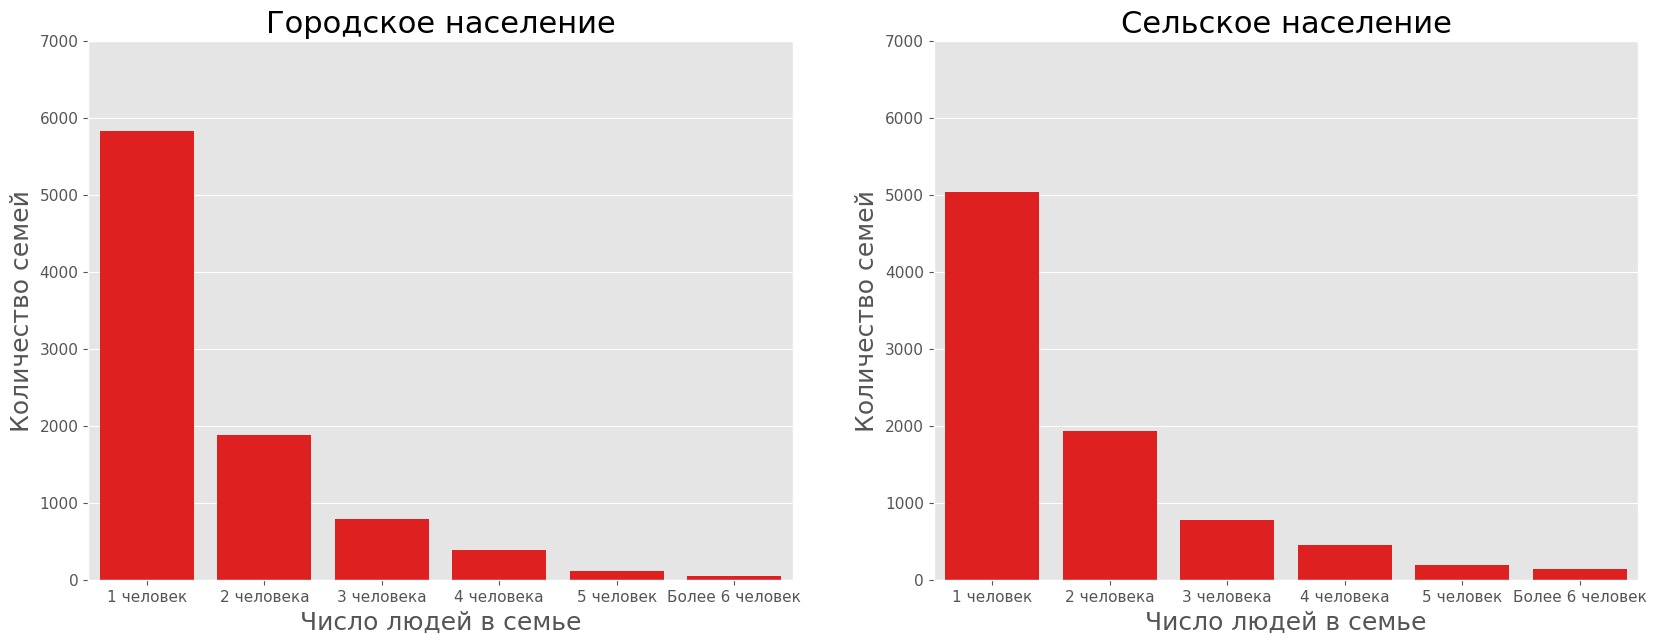
\includegraphics[width=1.\textwidth]{img/households_distibution_generated.png}
	\caption{Распределение домохозяйств для синтетической популяции размером 30000.}
	\label{fig:households_distibution_generated}
\end{figure}

На следующем этапе начинается процесс создание контактов внутри предприятий, школ и университетов. Сначала рассматриваются школы, число школ определяется исходя из размера популяции и данных, собранных на первом этапе. Контакты внутри школ формируются по модели <<small-world>> \cite{Watts}. Моделирование контактов данным алгоритмом происходит отдельно внутри каждого класса. Размер классов устанавливается заранее и не превышает 30 человек. Аналогичным образом происходит моделирование контактов внутри университетов, там рассматривается взаимодействие студентов в рамках групп. Результат работы алгоритма построения контактов внутри группы студентов приведен на рисунке \ref{fig:graph_connections}.

\begin{figure}[h!]
	\centering
	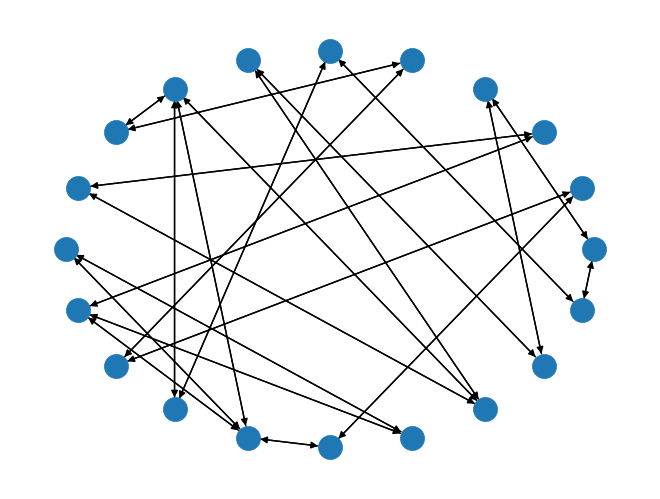
\includegraphics[width=0.5\textwidth]{img/graph_connections.png}
	\caption{Пример построения сети контактов внутри студенческой группы по модели <<small-world>>.}
	\label{fig:graph_connections}
\end{figure}

 Отдельного внимания заслуживает процесс моделирования контактов внутри предприятий. Здесь необходимо учитывать, что все предприятия имеют разный размер, а значит их надо моделировать особым образом. В решения был использован подход описанный в статье \cite{Axtell}. При таком способе моделирования число предприятий убывает линейно с увеличением их размера. Результат работы функции для создания предприятий нужных размеров приведен на рисунке \ref{fig:manufactories_linear}.

\begin{figure}[h!]
	\centering
	
\includegraphics[width=0.5\textwidth]{img/manufactoris_distribution.png}
	\caption{Распределение размеров предприятий по размерам.}
	\label{fig:manufactories_linear}
\end{figure}

При этом функция создания предприятий на вход получает параметр, который отвечает за то, сколько будет самых крупных предприятий. Если с таким число выполнить моделирование невозможно, алгоритм автоматически находит ближайшее допустимое значение к заданному, при этом на экран выводится сообщение с предупреждением.

Помимо этого в программе так же предусмотрен способ моделирования в режиме локдауна. В этом случает считается, что работать на предприятия ходит только 30\% от общего числа трудоспособного населения.

\textit{Моделирование распространения инфекции}.
После создания искуственной популяции с заданными параметрами на матрицах контактов для городского и сельского населений были построены графы, в которых каждая вершина -- конкретный человек, а его контакты -- связи между вершинами графа, по которым может распространяться инфекция. На полученных графах были рассчитаны степени вершин, таким образом исходная популяция была разбита на подгруппы, где члены каждой подгруппы имели одинаковое число контактов. Гистограммы распределения степеней вершин для городского и сельского населений представлены на рисунке \ref{fig:nodes_degrees}.

\begin{figure}[h!]
	\begin{minipage}{0.5\textwidth}
		\centering
		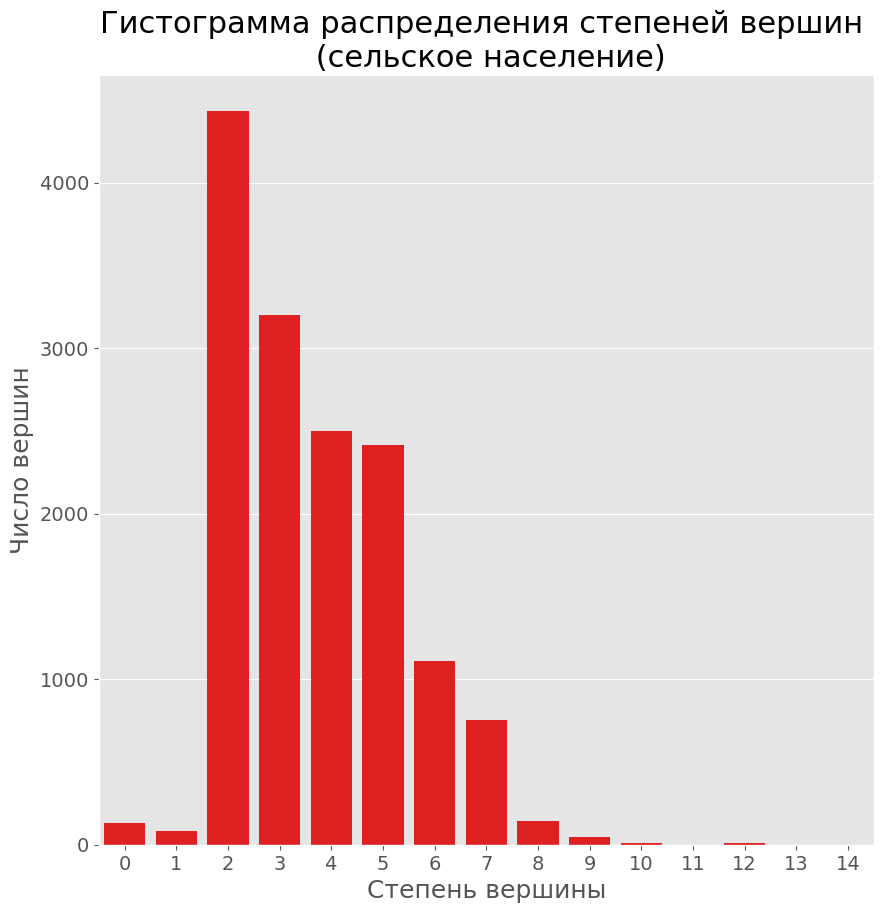
\includegraphics[width=\linewidth]{img/nodes_degrees_rural.png}
	\end{minipage}
	\begin{minipage}{0.5\textwidth}
		\centering
		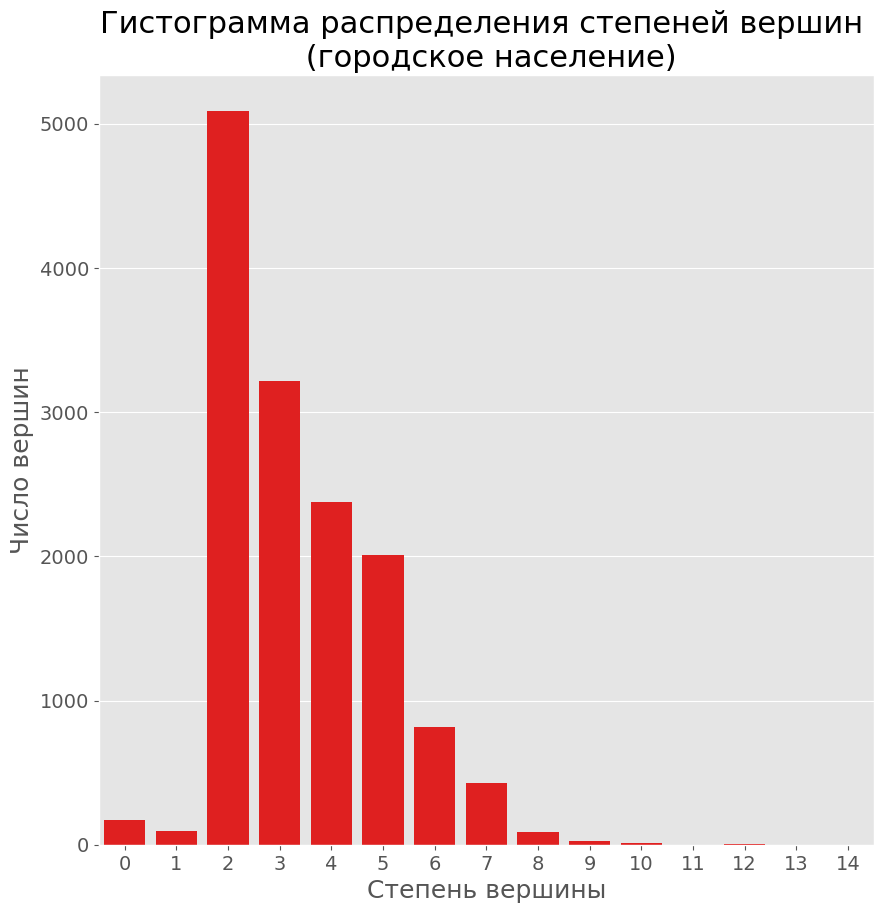
\includegraphics[width=\linewidth]{img/nodes_degrees_urban.png}
	\end{minipage}
	\label{fig:nodes_degrees}
	\caption{Распределение степеней вершин сгенерированной популяции для городского и сельского населений.}
\end{figure}

После этого к полученным подгруппам была применена SIR модель. На рисунке \ref{fig:sir_model_example} приведены графики изменения числа зараженных, выздоровевших и инфицированных с течением времени. В данном случае были взяты следующие параметры: $\gamma = 0.05, \beta_0 = 2$, тип популяции -- urban, размер популяции -- 100000, рассмотрена группа людей, имеющтх 12 контактов.

\begin{figure}[h!]
	\centering
	
\includegraphics[width=1.0\textwidth]{img/sir_model_example.png}
	\caption{Графики основных функций SIR модели для группы людей с 12 контактами.}
	\label{fig:sir_model_example}
\end{figure}

Так как в программе присутствуют методы, в основе которых содержится элементы случайности (например, в модели <<small-world>> случайным образом выбираются связи, которые будут разорваны), была предсмотрена возможность фиксации случайного состояния. При  таком подходе результаты работы алгоритма не отличаются от запуска к запуску.

\section{Эксперименты}
\subsection{Локдаун} 
Одним из основных способов борьбы с распространением инфекции является локдаун.
Под локдауном обычно понимается ряд строгих ограничений, которые вводит правительство, с целью предотвращения распространения вируса. Локдаун включает в себя закрытие школ, предприятий, магазинов, запрет на выход на улицу без необходимости.
Прежде всего такие меры помогают снизить количество контактов между людьми и их скопление в общественных местах. В реальных условиях такие меры также помогает медицинской системе снизить нагрузку на больницы и персонал.

В нашей модели наличие локдауна означает, что на предприятия ходят только 30\% трудоспособного населения. При этом отдельно были рассмотрены именно графики для инфицированных людей с целью оценки динамики распространения инфекции. Параметры, использованные при моделировании, приведены в таблице \ref{fig:table_paremeters}. Результаты работы алгоритма приведены на рисунке \ref{fig:nodes_degrees}.

\begin{figure}[h!]
	\begin{minipage}{0.5\textwidth}
		\centering
		\includegraphics[width=\linewidth]{img/sir_model_lockdown.png}
	\end{minipage}
	\begin{minipage}{0.5\textwidth}
		\centering
		\includegraphics[width=\linewidth]{img/sir_model_nonlockdown.png}
	\end{minipage}
	\label{fig:nodes_degrees}
	\caption{Динамика числа инфицированных людей с течением времени для случая локдауна (справа), и без него (слева).}
\end{figure}

\begin{table}[h]
	\centering
	\begin{tabular}{|c|c|c|c|c|}
		\hline
		Параметр & Gamma $(\gamma)$ & Beta\_0 ($\beta_0$) & Размер популяции & Тип популяции \\
		\hline
		Значение & $1/20$ & $10.0$ & $100000$ & Urban \\
		\hline
	\end{tabular}
	\label{fig:table_paremeters}
\caption{Таблица значений параметров, использованных для моделирования влияния локдауна на распространение инфекции.}
\end{table}

В ходе эксперимента было установлено, что без введения локдауна заболеванию подверглось 84\% населения, тогда как при введении локдауна -- 61\%.

Так же важным элементом оценки динамики распространения инфекции является знание периода, после которого начинается спад числа новых заражений. С программной точки зрения это значение  необходимо было оценить в разрезе групп людей с разным числом контактов и, как следствие, разными параметрами $\beta_k$. Для это было взято средневзвешенное по размеру группы значение  $\beta_k$. Для значения параметров из таблицы \ref{fig:table_paremeters} было получено $\beta_k$ = 0.68.

\section{Заключение}

В ходе реботы были собранны и проанализированны данные, необходимые для создания искуственной популяции. К ним относится информация о возростно-половом составе населения, распределение размеров домохозяйств, предприятий и учебных заведений. Был разработан алгоритм создания синтетических популяций с заданными характеристиками. При написании алгоритма использовались общеисзветные подходы, такие как модель контактов <<small-world>> и линейная зависимость размера предприятия от общего числа. В итоге была получена популяция с характеристиками близкими к реальным. По ее матрице контактов был построен граф, в котором каждый человек -- это вершина, а его связи -- это пути по которым может распространяться инфекция. Для всех вершин были посчитаны их степени, по которым все популяция далее разбилась на группы. На полученных группах была применена SIR модель распространения инфекции. При этом для решения системы дифференциальных уравнений были использованы методы численного интегрирования. После этого были проведены два эксперимента по оценки скорости распространения инфекции с использование локдауна и без. Было установлено, что при налиции локдауна переболел 61 \% населения, тогда как без него -- 86\%. При этом спад распространения инфекции при локдауне составил 28 дней а без 56. Полученные результаты соответствуют теоретическим ожиданиям. 
Созданный программный код является простым в использовании, имеет много доступных настроек и может быть использован для более детального изучения динамики распространения инфекции.

\section{Приложения}


\definecolor{lightblue}{RGB}{153,204,255}
\definecolor{darkblue}{RGB}{51,102,204}

\begin{table}[h!]
	\centering
	\setlength{\arrayrulewidth}{1pt}
	\renewcommand{\arraystretch}{1.5}
	\begin{tabularx}{\linewidth}{|X|X|X|X|X|}
		\hline
		{\cellcolor{lightblue}\textbf{Возрастная группа}} & 
		{\cellcolor{lightblue}\textbf{Мужчины (город)}} &
		{\cellcolor{lightblue}\textbf{ Женщины (город)}} &
		{\cellcolor{lightblue}\textbf{Мужчины (село)}}   &
		{\cellcolor{lightblue}\textbf{ Женщины (село)}} \\
		\hline
		0 – 4 & 0.048228 & 0.038131 & 0.041090 & 0.035985 \\ \hline
		05 – 9 & 0.065078 & 0.051348 & 0.057092 & 0.049954 \\ \hline
		10 - 14 & 0.060426 & 0.047758 & 0.057801 & 0.050684 \\ \hline
		15 - 19 & 0.057738 & 0.043964 & 0.048541 & 0.041152 \\ \hline
		20 - 24 & 0.052066 & 0.039552 & 0.044843 & 0.034962 \\ \hline
		25 - 29 & 0.055083 & 0.046135 & 0.051216 & 0.040149 \\ \hline
		30 - 34 & 0.087438 & 0.075185 & 0.078978 & 0.063005 \\ \hline
		35 - 39 & 0.094538 & 0.083253 & 0.084348 & 0.069109 \\ \hline
		40 - 44 & 0.084593 & 0.076494 & 0.077282 & 0.066098 \\ \hline
		45 - 49 & 0.075172 & 0.070111 & 0.074774 & 0.067012 \\ \hline
		50 - 54 & 0.062727 & 0.061496 & 0.072401 & 0.067978 \\ \hline
		55 - 59 & 0.062977 & 0.068045 & 0.082824 & 0.082579 \\ \hline
		60 - 64 & 0.067163 & 0.081208 & 0.091281 & 0.097663 \\ \hline
		65 - 69 & 0.054906 & 0.075574 & 0.065990 & 0.081770 \\ \hline
		70 - 74 & 0.038728 & 0.060998 & 0.039667 & 0.059454 \\ \hline
		75 - 79 & 0.013435 & 0.025484 & 0.011941 & 0.024921 \\ \hline
		80 - 84 & 0.013622 & 0.035173 & 0.013374 & 0.040230 \\ \hline
		85 и более & 0.006083 & 0.020092 & 0.006556 & 0.027296 \\
		\hline
	\end{tabularx}
	\caption{Таблица коэффициентов $\alpha$ по возрастным группам для города и сельской местности.}
	\label{coeff}
\end{table}


\definecolor{lightblue}{RGB}{153,204,255}
\definecolor{darkblue}{RGB}{51,102,204}

\begin{table}[h!]
	\centering
	\setlength{\arrayrulewidth}{1pt}
	\renewcommand{\arraystretch}{1.5}
	\begin{tabularx}{\linewidth}{|X|X|X|X|X|}
		\hline
		{\cellcolor{lightblue}\textbf{\small Возрастная группа}} &
		{\cellcolor{lightblue}\textbf{\small Работающие городские мужчины}} &
		{\cellcolor{lightblue}\textbf{\small Работающие сельские мужчины}}  & 
		{\cellcolor{lightblue}\textbf{\small Работающие городские женщины}} &
		{\cellcolor{lightblue}\textbf{\small Работающие сельские женщины}}  \\ \hline
		15-19 & 0.007213 & 0.007326 & 0.007216 & 0.007605 \\ \hline
		20-29 & 0.151962 & 0.153703 & 0.130307 & 0.132786 \\ \hline
		30-39 & 0.304655 & 0.283241 & 0.284305 & 0.265716 \\ \hline
		40-49 & 0.261809 & 0.252996 & 0.284548 & 0.287475 \\ \hline
		50-59 & 0.190951 & 0.223993 & 0.207252 & 0.235805 \\ \hline
		60-69 & 0.075921 & 0.074554 & 0.076101 & 0.064979 \\ \hline
		70-74 & 0.005512 & 0.003359 & 0.007223 & 0.004248 \\ \hline
		75 and over & 0.001977 & 0.000827 & 0.003048 & 0.001386 \\ \hline
	\end{tabularx}
	\caption{Таблица коэффициентов $\beta$  работающих людей по возрастным группам для города и сельской местности.}
	\label{coeffааа}
\end{table}


\definecolor{lightblue}{RGB}{153,204,255}
\definecolor{darkblue}{RGB}{51,102,204}

\begin{table}[h!]
	\centering
	\setlength{\arrayrulewidth}{1pt}
	\renewcommand{\arraystretch}{1.5}
	\begin{tabularx}{\linewidth}{|X|X|X|}
		
		\hline
		{\cellcolor{lightblue}\textbf{\small Размер домохозяйства, (число человек)}}& {\cellcolor{lightblue}\textbf{\small Доля от общего числа домохозяйств для сельского населения, (\%)}}&
		{\cellcolor{lightblue}\textbf{\small Доля от общего числа домохозяйств для сельского населения, (\%)}} \\
		\hline
		1 & 34.5 & 43.2  \\
		\hline
		2 & 25.8 & 25.2  \\
		\hline
		3 & 15.6 & 15.8  \\
		\hline
		4 & 12.2 & 10.3  \\
		\hline
		5 & 6.4 & 3.6  \\
		\hline
		более 6 & 5.5 & 1.9  \\
		\hline
	\end{tabularx}
	
	\caption{Размеры домохозяйств для городского и сельского населений, усредненное по регионам страны  \cite{rosstat}.}
	\label{tab: 111}
\end{table}



\newpage


\begin{thebibliography}{99}
	\bibitem{Murray} Murray J. D., Murray J. D. Epidemic models and the dynamics of infectious diseases //Mathematical biology. – 1993. – С. 610-650.
	\bibitem{Tomsk} Ajelli M., Litvinova M. Estimating contact patterns relevant to the spread of infectious diseases in Russia //Journal of theoretical biology. – 2017. – Т. 419. – С. 1-7.
	
	\bibitem{network_analysis} Klovdahl A. S. et al. Social Networks in an Urban Area: First Canberra Study1 //The Australian and New Zealand Journal of Sociology. – 1977. – Т. 13. – №. 2. – С. 169-172.
	
	\bibitem{Klovdahl} Klovdahl A. S. et al. Social Networks in an Urban Area: First Canberra Study1 //The Australian and New Zealand Journal of Sociology. – 1977. – Т. 13. – №. 2. – С. 169-172.
	
	\bibitem{Eubank} Eubank S. et al. Modelling disease outbreaks in realistic urban social networks //Nature. – 2004. – Т. 429. – №. 6988. – С. 180-184.
	
	\bibitem{Meyers} Meyers L. A. et al. Network theory and SARS: predicting outbreak diversity //Journal of theoretical biology. – 2005. – Т. 232. – №. 1. – С. 71-81.
	
	\bibitem{Meyers_2003} Meyers L. A. et al. Applying network theory to epidemics: control measures for Mycoplasma pneumoniae outbreaks //Emerging infectious diseases. – 2003. – Т. 9. – №. 2. – С. 204.

	\bibitem{Halloran} Halloran M. E. et al. Containing bioterrorist smallpox //Science. – 2002. – Т. 298. – №. 5597. – С. 1428-1432.

	\bibitem{BA} Barabási A. L., Albert R. Emergence of scaling in random networks //science. – 1999. – Т. 286. – №. 5439. – С. 509-512.

	\bibitem{Watts}	Watts D. J., Strogatz S. H. Collective dynamics of ‘small-world’networks //nature. – 1998. – Т. 393. – №. 6684. – С. 440-442.
	
	\bibitem{www} Jeong A. H. Diameter of the world-wide web //Nature. – 1999. – Т. 401. – С. 130-131.
	
	\bibitem{Wuchty}
	Wuchty S. Scale-free behavior in protein domain networks //Molecular biology and evolution. – 2001. – Т. 18. – №. 9. – С. 1694-1702.
	
	\bibitem{rosstat} https://rosstat.gov.ru/
	\bibitem{github} dfdf
	
	\bibitem{Axtell} Axtell R. L. Zipf distribution of US firm sizes //science. – 2001. – Т. 293. – №. 5536. – С. 1818-1820.
	
	
\end{thebibliography}

\end{document}

